\section{Differentialgleichungssysteme 1. Ordnung}

\subsection{Einführungsbeispiel}

Wir betrachten zwei verbundene Behälter, welche beide ein Gemisch aus
Farbstoff und Wasser enthalten.
\begin{center}
    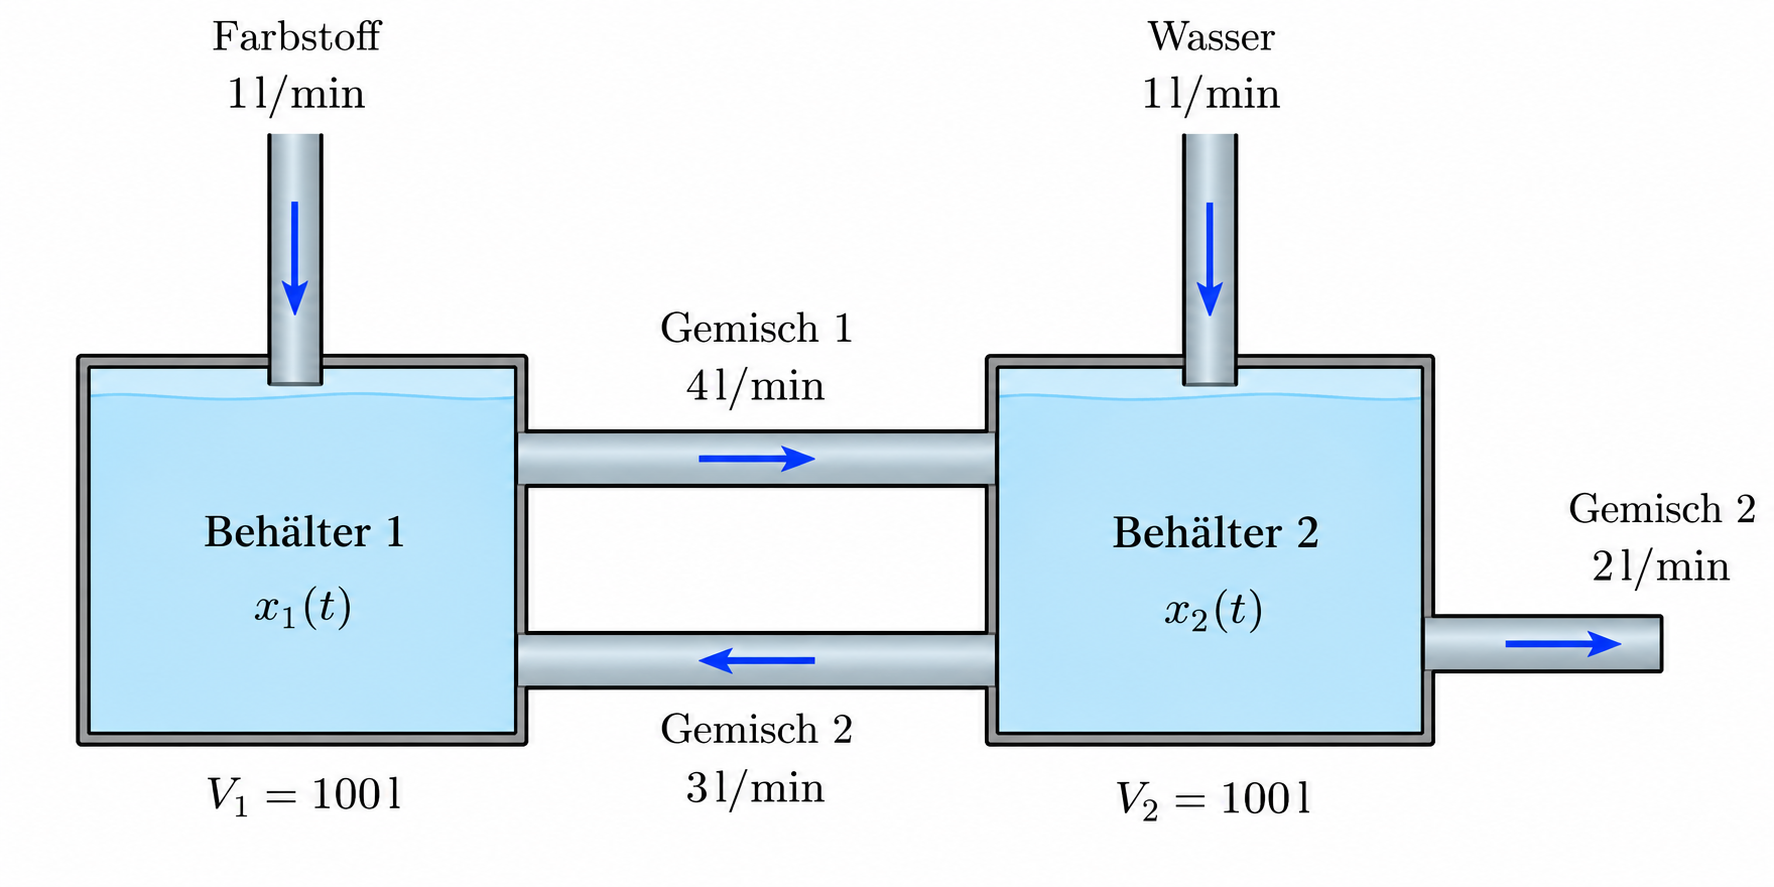
\includegraphics[width = 0.75\textwidth]{media/Schematische Zwei-Tank-Mischanlage.png}
\end{center}
% \begin{center}
%     \begin{tikzpicture}[
%             >=stealth,
%             thick,
%             flow/.style={->, very thick},
%             every node/.style={font=\small}
%         ]

%         % Abmessungen
%         \def\W{3.5}
%         \def\H{2.5}

%         % Wasserfüllungen
%         \fill[cyan!12] (0,0) rectangle (\W,\H);
%         \fill[cyan!12] (7,0) rectangle (7+\W,\H);

%         % Behälter (oben offen)
%         \draw (0,\H) -- (0,0) -- (\W,0) -- (\W,\H) -- (0,\H);
%         \draw (7,\H) -- (7,0) -- (7+\W,0) -- (7+\W,\H) -- (7,\H);

%         % Beschriftungen
%         \node at (1.75,1.2) {\textbf{Behälter 1}};
%         \node at (1.75,0.7) {\(x_1(t)\)};
%         \node at (8.75,1.2) {\textbf{Behälter 2}};
%         \node at (8.75,0.7) {\(x_2(t)\)};

%         % Zufluss Farbstoff
%         \draw[flow,blue!70!black] (1.75,4.0) -- (1.75,2.0);
%         \node[above,align=center] at (1.75,4.0)
%         {Farbstoff\\ \(\SI{1}{\liter\per\minute}\)};

%         % Zufluss Wasser
%         \draw[flow,blue!70!black] (8.75,4.0) -- (8.75,2.0);
%         \node[above,align=center] at (8.75,4.0)
%         {Wasser\\ \(\SI{1}{\liter\per\minute}\)};

%         % Verbindung Behälter 1 -> Behälter 2
%         \draw[flow] (3.5,1.8) -- (7,1.8);
%         \node[above,align=center] at (5.25,1.8)
%         {Gemisch 1\\ \(\SI{4}{\liter\per\minute}\)};

%         % Verbindung Behälter 2 -> Behälter 1
%         \draw[flow] (7,0.45) -- (3.5,0.45);
%         \node[below,align=center] at (5.25,0.45)
%         {Gemisch 2\\ \(\SI{3}{\liter\per\minute}\)};

%         % Abfluss Behälter 2
%         \draw[flow] (10.5,1.2) -- (12.7,1.2);
%         \node[right,align=left] at (12.7,1.2)
%         {Gemisch 2\\ \(\SI{2}{\liter\per\minute}\)};

%         % Volumenangaben
%         \node[below] at (1.75,-0.1) {\(V_1=\SI{100}{\liter}\)};
%         \node[below] at (8.75,-0.1) {\(V_2=\SI{100}{\liter}\)};

%     \end{tikzpicture}
% \end{center}
Dabei werden folgende Annahmen gemacht:

\begin{enumerate}
    \item In beiden Behältern wird ständig gerührt, sodass die
          Gemische homogen gehalten werden.

    \item Zur Zeit \(t=0\) enthalten beide Behälter
          \(\SI{100}{\liter}\) reines Wasser.
          Da in beiden Behältern gleich viele Liter abgepumpt
          wie zugeführt werden, befinden sich zu jedem
          Zeitpunkt jeweils \(\SI{100}{\liter}\) in den Behältern.
\end{enumerate}

Seien
\begin{align*}
    x_1(t) & : \text{Farbstoffmenge in Litern im ersten Behälter
                   zur Zeit } t,  \\
    x_2(t) & : \text{Farbstoffmenge in Litern im zweiten Behälter
                   zur Zeit } t.
\end{align*}

Damit haben wir die Anfangsbedingungen
\[
    x_1(0)=x_2(0)=0.
\]

Nun ermitteln wir analog zum Beispiel des Salzwassertanks
eine Differentialgleichung für \(x_1\) und \(x_2\).

Wiederum überlegen wir uns, wie sich der Farbstoffgehalt
in einer sehr kurzen Zeitspanne \(h\) verändert.
\clearpage
\karofeld{7}
Wir erhalten daher die Differentialgleichung
\[
    \dot{x}_1
    = -\frac{1}{25}x_1
    + \frac{3}{100}x_2
    + 1.
\]

Analog erhalten wir für \(x_2\) die Differentialgleichung
\[
    \dot{x}_2
    = \frac{1}{25}x_1
    - \frac{1}{20}x_2.
\]

Da beide Differentialgleichungen nicht getrennt voneinander
gelöst werden können, spricht man auch von
\emph{gekoppelten Differentialgleichungen}.

Wir haben also ein System von zwei Differentialgleichungen:
\[
    \left\{
    \begin{aligned}
        \dot{x}_1 & = -\frac{1}{25}x_1
        + \frac{3}{100}x_2 + 1,        \\
        \dot{x}_2 & = \frac{1}{25}x_1
        - \frac{1}{20}x_2.
    \end{aligned}
    \right.
\]

Dieses System lässt sich auch mithilfe von Matrizen und
Vektoren schreiben:
\[
    \begin{pmatrix}
        \dot{x}_1 \\
        \dot{x}_2
    \end{pmatrix}
    =
    \begin{pmatrix}
        -\frac{1}{25} & \frac{3}{100} \\
        \frac{1}{25}  & -\frac{1}{20}
    \end{pmatrix}
    \begin{pmatrix}
        x_1 \\
        x_2
    \end{pmatrix}
    +
    \begin{pmatrix}
        1 \\
        0
    \end{pmatrix}.
\]

Wir erhalten also ein Differentialgleichungssystem der Form
\[
    \frac{\mathrm{d}}{\mathrm{d}t}\vec{x}
    = A\vec{x}+\vec{b}.
\]

In Anlehnung an die Terminologie der einfachen
Differentialgleichungen bezeichnet man dieses System als
\emph{inhomogenes lineares Differentialgleichungssystem
    erster Ordnung}.





























\clearpage
\subsection{Homogene lineare Differentialgleichungssysteme erster Ordnung}

Wir betrachten Systeme von der Form
\[
    \frac{\mathrm{d}}{\mathrm{d}t}\vec{x}=A\vec{x}.
\]

Auch für homogene Differentialgleichungssysteme erster Ordnung gilt das Superpositionsprinzip:

\begin{satz}{Superpositionsprinzip}{}
    Seien \(\vec{x}_1\) und \(\vec{x}_2\) zwei Lösungen des Differentialgleichungssystems
    \[
        \frac{\mathrm{d}}{\mathrm{d}t}\vec{x}=A\vec{x}.
    \]
    Dann ist auch
    \[
        \vec{x}=c_1\vec{x}_1+c_2\vec{x}_2
    \]
    für jede Wahl von \(c_1,c_2\in\mathbb{R}\) eine Lösung dieses Systems.
\end{satz}

Da die Lösung einer Differentialgleichung erster Ordnung einen Freiheitsgrad aufweist (die frei wählbare Konstante), sind bei einem System aus \(n\) Differentialgleichungen erster Ordnung insgesamt \(n\) Freiheitsgrade zu erwarten.

\begin{satz}{}{}
    Das Differentialgleichungssystem
    \[
        \frac{\mathrm{d}}{\mathrm{d}t}\vec{x}=A\vec{x}
    \]
    mit der \(2\times 2\)-Matrix \(A\) besitzt zwei linear unabhängige Fundamentallösungen \(\vec{x}_1\) und \(\vec{x}_2\).

    Die allgemeine Lösung des Differentialgleichungssystems lautet dann
    \[
        \vec{x}=c_1\vec{x}_1+c_2\vec{x}_2.
    \]
\end{satz}

Wir betrachten Differentialgleichungssysteme
\[
    \frac{\mathrm{d}}{\mathrm{d}t}\vec{x}=A\vec{x}
\]
mit einer \(2\times 2\)-Matrix \(A\). In diesem Fall brauchen wir zwei linear unabhängige Fundamentallösungen. Die Menge aller Linearkombinationen dieser beiden Fundamentallösungen ist dann die allgemeine Lösung des homogenen Differentialgleichungssystems.

Wie finden wir nun diese Fundamentallösungen?



\subsubsection{Diagonale oder diagonalisierbare Matrizen}

\textbf{Ist die Matrix \(A\) eine Diagonalmatrix}, so sind die einzelnen Differentialgleichungen entkoppelt und wir können sie mit den gelernten Methoden einzeln lösen:

\[
    \begin{pmatrix}
        \dot{x}_1 \\
        \dot{x}_2
    \end{pmatrix}
    =
    \begin{pmatrix}
        2 & 0 \\
        0 & 3
    \end{pmatrix}
    \begin{pmatrix}
        x_1 \\
        x_2
    \end{pmatrix}
    \quad\Longleftrightarrow\quad
    \left\{
    \begin{aligned}
        \dot{x}_1 & = 2x_1 \\
        \dot{x}_2 & = 3x_2
    \end{aligned}
    \right.
\]

Damit ist \(x_1=c_1e^{2t}\) und \(x_2=c_2e^{3t}\), oder in Matrixschreibweise zusammengefasst:

\[
    \begin{pmatrix}
        x_1 \\
        x_2
    \end{pmatrix}
    =
    c_1
    \begin{pmatrix}
        1 \\
        0
    \end{pmatrix}
    e^{2t}
    +
    c_2
    \begin{pmatrix}
        0 \\
        1
    \end{pmatrix}
    e^{3t}.
\]

Die allgemeine Lösung dieses Spezialfalls ergibt sich also als Linearkombination der beiden Fundamentallösungen
\[
    \begin{pmatrix}
        1 \\
        0
    \end{pmatrix}e^{2t}
    \qquad\text{und}\qquad
    \begin{pmatrix}
        0 \\
        1
    \end{pmatrix}e^{3t}.
\]

\medskip

\textbf{Falls die Matrix \(A\) nicht diagonal ist}, helfen uns die Erkenntnisse aus der linearen Algebra.

Nehmen wir einmal an, dass \(A\) zwei unterschiedliche Eigenwerte \(\lambda_1\) und \(\lambda_2\) mit den dazugehörigen Eigenvektoren
\[
    \vec{v}_1=
    \begin{pmatrix}
        a_1 \\
        a_2
    \end{pmatrix}
    \qquad\text{und}\qquad
    \vec{v}_2=
    \begin{pmatrix}
        b_1 \\
        b_2
    \end{pmatrix}
\]
hat.

Diese bilden eine neue Basis
\[
    \mathcal{B}=(\vec{v}_1,\vec{v}_2),
\]
bezüglich welcher das Differentialgleichungssystem entkoppelt ist.

Mit der Transformationsmatrix
\[
    T=
    \begin{pmatrix}
        a_1 & b_1 \\
        a_2 & b_2
    \end{pmatrix}
\]
hat man dann das folgende Schema:
% Benötigt: \usepackage{xcolor,amsmath}

\[
    \begin{array}{ccc}
        {\color{green!65!black}
            \begin{pmatrix} y_1 \\ y_2 \end{pmatrix}_{\mathcal{B}}}
         &
        {\color{green!65!black}
            \xrightarrow{\quad
                D=\begin{pmatrix}
                    \lambda_1 & 0         \\
                    0         & \lambda_2
                \end{pmatrix}
                \quad}}
         &
        {\color{green!65!black}
            \begin{pmatrix} \dot y_1 \\ \dot y_2 \end{pmatrix}_{\mathcal{B}}}
        \\[1.5em]
        \Big\downarrow T
         &   &
        \Big\uparrow T^{-1}
        \\[1.5em]
        {\color{red}
            \begin{pmatrix} x_1 \\ x_2 \end{pmatrix}_{\mathcal{S}t}}
         &
        {\color{red}\xrightarrow{\quad A\quad}}
         &
        {\color{red}
            \begin{pmatrix} \dot x_1 \\ \dot x_2 \end{pmatrix}_{\mathcal{S}t}}
    \end{array}
\]

In dieser Basis aus Eigenvektoren (obere Zeile des Schemas)
lässt sich das Differentialgleichungssystem leicht lösen.
Es gilt:
\[
    {\color{green!65!black}
        \vec{y}
        = c_1
        \begin{pmatrix}1\\0\end{pmatrix}e^{\lambda_1t}
        + c_2
        \begin{pmatrix}0\\1\end{pmatrix}e^{\lambda_2t}.}
\]

Um die Lösung der ursprünglichen Differentialgleichung zu finden,
muss man schliesslich die Basistransformation rückgängig machen.

\[
    \begin{aligned}
        {\color{red}\vec{x}}
         & = T\cdot{\color{green!65!black}\vec{y}}                         \\
         & = T\cdot\left(
                   {\color{green!65!black}
                       c_1\begin{pmatrix}1\\0\end{pmatrix}e^{\lambda_1t}
                       +c_2\begin{pmatrix}0\\1\end{pmatrix}e^{\lambda_2t}}
        \right)                                                            \\
         & = c_1T\begin{pmatrix}1\\0\end{pmatrix}e^{\lambda_1t}
        +c_2T\begin{pmatrix}0\\1\end{pmatrix}e^{\lambda_2t}                \\
         & = {\color{red}
                 c_1\vec{v}_1e^{\lambda_1t}
                 +c_2\vec{v}_2e^{\lambda_2t}}.
    \end{aligned}
\]

Die allgemeine Lösung dieses Spezialfalls ergibt sich also
als Linearkombination der beiden Fundamentallösungen
\[
    \vec{v}_1e^{\lambda_1t}
    \qquad\text{und}\qquad
    \vec{v}_2e^{\lambda_2t}.
\]

Etwas allgemeiner als Satz formuliert:

\begin{satz}{}{}
    Sei \(\vec{v}\) ein Eigenvektor der Matrix \(A\) zum
    Eigenwert \(\lambda\). Dann ist
    \[
        \vec{x}(t)=\vec{v}\,e^{\lambda t}
    \]
    eine Lösung des Differentialgleichungssystems
    \[
        \frac{\mathrm{d}}{\mathrm{d}t}\vec{x}=A\vec{x}.
    \]
\end{satz}

\textbf{Beweis:}
Wir können durch Einsetzen prüfen, ob
\(\vec{x}=\vec{v}e^{\lambda t}\) tatsächlich eine Lösung ist:

\[
    \begin{aligned}
        \frac{\mathrm{d}}{\mathrm{d}t}\vec{x}
         & =\frac{\mathrm{d}}{\mathrm{d}t}
        \left(\vec{v}e^{\lambda t}\right)      \\
         & =\vec{v}\lambda e^{\lambda t}       \\
         & =(\lambda\vec{v})e^{\lambda t}      \\
         & =(A\vec{v})e^{\lambda t}            \\
         & =A\left(\vec{v}e^{\lambda t}\right) \\
         & =A\vec{x}.
    \end{aligned}
\]

Wenn wir mithilfe der Eigenwerttheorie also zwei linear
unabhängige Lösungen von der Form
\(\vec{v}e^{\lambda t}\) gefunden haben, dann ist die Menge
aller Linearkombinationen dieser beiden Fundamentallösungen
die Lösungsmenge des Differentialgleichungssystems.

Nicht immer finden wir direkt mithilfe der Eigenwerttheorie
zwei linear unabhängige Fundamentallösungen.
Auf solche Fälle kommen wir später zurück.


\begin{bsp}{Differentialgleichungssystem lösen}{}

    Gegeben ist das Differentialgleichungssystem
    \[
        \frac{\mathrm{d}}{\mathrm{d}t}\vec{x}
        =
        \begin{pmatrix}
            1 & 1 \\
            4 & 1
        \end{pmatrix}
        \vec{x}.
    \]

    Wir bestimmen also die Eigenwerte und die Eigenvektoren der Matrix
    \[
        A=
        \begin{pmatrix}
            1 & 1 \\
            4 & 1
        \end{pmatrix}.
    \]

    \textbf{Eigenwerte:}

    \begin{align*}
        \det(A-\lambda E)
         & =
        \det
        \begin{pmatrix}
            1-\lambda & 1         \\
            4         & 1-\lambda
        \end{pmatrix}  \\
         & =(1-\lambda)^2-4        \\
         & =\lambda^2-2\lambda-3   \\
         & =(\lambda-3)(\lambda+1)
        \stackrel{!}{=}0
    \end{align*}

    Damit erhalten wir
    \[
        \lambda_1=3,
        \qquad
        \lambda_2=-1.
    \]

    \textbf{Eigenvektor zum Eigenwert \(\lambda_1=3\):}

    \[
        \begin{aligned}
            \begin{pmatrix}
                1 & 1 \\
                4 & 1
            \end{pmatrix}
            \begin{pmatrix}a\\b\end{pmatrix}
             & =
            3\begin{pmatrix}a\\b\end{pmatrix} \\
             & \Longleftrightarrow
            \begin{cases}
                -2a+b=0 \\
                4a-2b=0
            \end{cases}                  \\
             & \Longleftrightarrow b=2a
        \end{aligned}
    \]

    Somit ist
    \[
        \vec{v}_1=k
        \begin{pmatrix}
            1 \\2
        \end{pmatrix},
        \qquad k\in\mathbb{R}\setminus\{0\}.
    \]

    \textbf{Eigenvektor zum Eigenwert \(\lambda_2=-1\):}

    \[
        \begin{aligned}
            \begin{pmatrix}
                1 & 1 \\
                4 & 1
            \end{pmatrix}
            \begin{pmatrix}a\\b\end{pmatrix}
             & =
            -\begin{pmatrix}a\\b\end{pmatrix} \\
             & \Longleftrightarrow
            \begin{cases}
                2a+b=0 \\
                4a+2b=0
            \end{cases}                  \\
             & \Longleftrightarrow b=-2a
        \end{aligned}
    \]

    Somit ist
    \[
        \vec{v}_2=k
        \begin{pmatrix}
            1 \\-2
        \end{pmatrix},
        \qquad k\in\mathbb{R}\setminus\{0\}.
    \]

    Die beiden Fundamentallösungen lauten folglich
    \[
        \vec{x}_1(t)=
        \begin{pmatrix}
            1 \\2
        \end{pmatrix}e^{3t}
        \qquad\text{und}\qquad
        \vec{x}_2(t)=
        \begin{pmatrix}
            1 \\-2
        \end{pmatrix}e^{-t}.
    \]

    Diese sind offensichtlich linear unabhängig.

    Damit lautet die allgemeine Lösung des
    Differentialgleichungssystems:
    \[
        \boxed{
            \begin{pmatrix}
                x_1(t) \\
                x_2(t)
            \end{pmatrix}
            =
            c_1
            \begin{pmatrix}
                1 \\2
            \end{pmatrix}e^{3t}
            +
            c_2
            \begin{pmatrix}
                1 \\-2
            \end{pmatrix}e^{-t}
        }
    \]

\end{bsp}

\begin{ueb}{Differentialgleichungssysteme}{}

    \begin{enumerate}
        \item Lösen Sie die folgenden DGL-Systeme allgemein:

              \begin{enumerate}
                  \item
                        \[
                            \frac{\mathrm{d}}{\mathrm{d}t}\vec{x}
                            =
                            \begin{pmatrix}
                                2 & 0  \\
                                0 & -2
                            \end{pmatrix}
                            \vec{x}
                        \]

                  \item
                        \[
                            \frac{\mathrm{d}}{\mathrm{d}t}\vec{x}
                            =
                            \begin{pmatrix}
                                -3       & \sqrt{2} \\
                                \sqrt{2} & -2
                            \end{pmatrix}
                            \vec{x}
                        \]
              \end{enumerate}

        \item Lösen Sie das folgende Anfangswertproblem:
              \[
                  \begin{cases}
                      \dot{x}_1=x_1+3x_2 \\
                      \dot{x}_2=2x_1+2x_2
                  \end{cases}
                  \qquad
                  x_1(0)=0,\quad x_2(0)=5
              \]

        \item Gegeben ist das DGL-System
              \[
                  \frac{\mathrm{d}}{\mathrm{d}t}\vec{x}
                  =
                  \begin{pmatrix}
                      -\frac{1}{2} & 1            \\
                      -1           & -\frac{1}{2}
                  \end{pmatrix}
                  \vec{x}.
              \]

              \begin{enumerate}
                  \item Bestimmen Sie die allgemeine komplexe Lösung des Systems.

                  \item In der komplexen Lösung sind auch zwei reelle,
                        linear unabhängige Lösungen enthalten.

                        Bestimmen Sie diese analog zu den gewöhnlichen
                        Differentialgleichungen zweiter Ordnung, indem Sie
                        \[
                            e^{(a+bi)t}
                            =
                            e^{at}\bigl(\cos(bt)+i\sin(bt)\bigr)
                        \]
                        verwenden.
              \end{enumerate}
    \end{enumerate}

\end{ueb}

\clearpage

\textbf{Lösungen:}

\begin{enumerate}
    \item Allgemeine Lösungen
          \begin{enumerate}
              \item
                    \[
                        \vec{x}(t)
                        = c_1 \begin{pmatrix} 1 \\ 0 \end{pmatrix} e^{2t}
                        + c_2 \begin{pmatrix} 0 \\ 1 \end{pmatrix} e^{-2t}
                    \]

              \item
                    \[
                        \vec{x}(t)
                        = c_1 \begin{pmatrix} 1 \\ \sqrt{2} \end{pmatrix} e^{-t}
                        + c_2 \begin{pmatrix} -\sqrt{2} \\ 1 \end{pmatrix} e^{-4t}
                    \]
          \end{enumerate}

    \item
          \[
              \vec{x}(t)
              = \begin{pmatrix} -3 \\ 2 \end{pmatrix} e^{-t}
              + \begin{pmatrix} 3 \\ 3 \end{pmatrix} e^{4t}
          \]

    \item Komplexe Eigenwerte
          \begin{enumerate}
              \item
                    \[
                        \vec{x}(t)
                        = c_1 \begin{pmatrix} 1 \\ i \end{pmatrix}
                        e^{\left(-\frac12+i\right)t}
                        + c_2 \begin{pmatrix} 1 \\ -i \end{pmatrix}
                        e^{\left(-\frac12-i\right)t},
                        \qquad c_1,c_2\in\mathbb{C}
                    \]

              \item
                    \[
                        \vec{x}(t)
                        = e^{-\frac12 t}
                        \left(
                        c_1 \begin{pmatrix} \cos t \\ -\sin t \end{pmatrix}
                        + c_2 \begin{pmatrix} \sin t \\ \cos t \end{pmatrix}
                        \right),
                        \qquad c_1,c_2\in\mathbb{R}
                    \]
          \end{enumerate}
\end{enumerate}




















\clearpage
\subsubsection{Nicht-diagonalisierbare Matrizen}
Wenn wir Eigenwerte und Eigenvektoren bestimmen, können folgende Fälle auftreten:

\begin{enumerate}
    \item \textbf{Beide Eigenwerte \(\lambda_1,\lambda_2\) sind reell und verschieden voneinander.}

          In diesem Fall sind die dazugehörigen Eigenvektoren
          \(\vec{v}_1\) und \(\vec{v}_2\) linear unabhängig.
          Die allgemeine Lösung lautet entsprechend
          \[
              \vec{x}(t)
              = c_1 \vec{v}_1 e^{\lambda_1 t}
              + c_2 \vec{v}_2 e^{\lambda_2 t}.
          \]

    \item \textbf{Die beiden Eigenwerte sind konjugiert komplexe Zahlen
              \(\lambda_{1,2}=a\pm bi\), \(a,b\in\mathbb{R}\).}

          Wenn die Eigenwerte komplex sind, müssen wir auch komplexe
          Eigenvektoren bestimmen. Die allgemeine komplexe Lösung lautet dann
          \[
              \vec{x}(t)
              = c_1 \vec{v}_1 e^{\lambda_1 t}
              + c_2 \vec{v}_2 e^{\lambda_2 t},
              \qquad c_1,c_2\in\mathbb{C}.
          \]

    \item \textbf{Genau ein (doppelter) Eigenwert \(\lambda\).}

          \begin{enumerate}
              \item \textbf{Matrix diagonalisierbar}

                    Wenn die Eigenvektoren der Matrix \(A\) die ganze Ebene
                    \(\mathbb{R}^2\) aufspannen, ist die Matrix diagonalisierbar.
                    Da nur ein Eigenwert \(\lambda\) vorliegt, ist die Matrix
                    in diesem Fall von der Form
                    \[
                        A=
                        \begin{pmatrix}
                            \lambda & 0       \\
                            0       & \lambda
                        \end{pmatrix}.
                    \]

                    Die allgemeine Lösung lautet:
                    \[
                        \vec{x}(t)
                        = c_1
                        \begin{pmatrix}1\\0\end{pmatrix}e^{\lambda t}
                        + c_2
                        \begin{pmatrix}0\\1\end{pmatrix}e^{\lambda t}
                        =
                        \begin{pmatrix}c_1\\c_2\end{pmatrix}e^{\lambda t}.
                    \]

              \item \textbf{Genau ein (doppelter) Eigenwert \(\lambda\),
                        Matrix nicht diagonalisierbar}

                    Etwas komplizierter ist es, wenn die Matrix nicht
                    diagonalisierbar ist. Es gibt aber immer zwei linear
                    unabhängige Fundamentallösungen. Wie finden wir also
                    die zweite, linear unabhängige Lösung?

                    Sei \(\vec{v}\) ein Eigenvektor der Matrix zum Eigenwert
                    \(\lambda\). Inspiriert vom Vorgehen bei
                    Differentialgleichungen 2. Ordnung könnte man versucht sein,
                    \[
                        \vec{x}(t)=t\vec{v}e^{\lambda t}
                    \]
                    als weitere Lösung zu vermuten.

                    Wie man aber leicht nachprüfen kann, ist dies keine Lösung:
                    \[
                        \begin{aligned}
                            \frac{\mathrm{d}}{\mathrm{d}t}
                            \left(t\vec{v}e^{\lambda t}\right)
                             & = \vec{v}e^{\lambda t}
                            +\lambda t\vec{v}e^{\lambda t}            \\
                             & \neq \lambda t\vec{v}e^{\lambda t}     \\
                             & = A\left(t\vec{v}e^{\lambda t}\right).
                        \end{aligned}
                    \]

                    Wie man sieht, ist mit diesem Ansatz nur ein Teil
                    der Gleichung erfüllt. Ein besserer Ansatz sieht deshalb
                    folgendermassen aus:
                    \[
                        \vec{x}(t)=(\vec{u}+t\vec{v})e^{\lambda t}.
                    \]

                    Dabei ist \(\lambda\) der mehrfach vorkommende Eigenwert
                    und \(\vec{v}\) der zugehörige Eigenvektor.
                    Der Vektor \(\vec{u}\) ist unbekannt und muss so bestimmt
                    werden, dass der Ansatz das DGL-System
                    \[
                        \frac{\mathrm{d}}{\mathrm{d}t}\vec{x}
                        = A\vec{x}
                    \]
                    löst.

                    Wir berechnen zunächst die Ableitung:
                    \[
                        \begin{aligned}
                            \frac{\mathrm{d}}{\mathrm{d}t}
                            \left((\vec{u}+t\vec{v})e^{\lambda t}\right)
                             & = \vec{v}e^{\lambda t}
                            +(\vec{u}+t\vec{v})\lambda e^{\lambda t}   \\
                             & = (\lambda\vec{u}+\vec{v})e^{\lambda t}
                            +t\lambda\vec{v}e^{\lambda t}.
                        \end{aligned}
                    \]

                    Andererseits gilt:
                    \[
                        \begin{aligned}
                            A\left((\vec{u}+t\vec{v})e^{\lambda t}\right)
                             & = A\vec{u}e^{\lambda t}
                            +tA\vec{v}e^{\lambda t}    \\
                             & = A\vec{u}e^{\lambda t}
                            +t\lambda\vec{v}e^{\lambda t}.
                        \end{aligned}
                    \]

                    Durch Gleichsetzen erhalten wir
                    \[
                        \begin{aligned}
                            A\vec{u}                & = \lambda\vec{u}+\vec{v} \\
                            A\vec{u}-\lambda\vec{u} & = \vec{v}                \\
                            (A-\lambda E)\vec{u}    & = \vec{v}.
                        \end{aligned}
                    \]

                    \textbf{Fazit:} Ist die \(2\times 2\)-Matrix \(A\)
                    nicht diagonalisierbar, so lautet die allgemeine Lösung
                    des Differentialgleichungssystems
                    \[
                        \frac{\mathrm{d}}{\mathrm{d}t}\vec{x}=A\vec{x}
                    \]
                    \[
                        \boxed{
                            \vec{x}(t)
                            = c_1\vec{v}e^{\lambda t}
                            + c_2(\vec{u}+t\vec{v})e^{\lambda t}
                        }
                    \]

                    Dabei ist \(\lambda\) der einzige Eigenwert von \(A\),
                    \(\vec{v}\) ein zugehöriger Eigenvektor und
                    \(\vec{u}\) eine Lösung der Gleichung
                    \[
                        (A-\lambda E)\vec{u}=\vec{v}.
                    \]
          \end{enumerate}
\end{enumerate}


\begin{bsp}{Differentialgleichungssystem mit doppeltem Eigenwert}{}

    Gegeben ist das Differentialgleichungssystem
    \[
        \frac{\mathrm{d}}{\mathrm{d}t}\vec{x}
        =
        \begin{pmatrix}
            1 & -1 \\
            1 & 3
        \end{pmatrix}
        \vec{x}.
    \]

    Wie immer bestimmen wir zuerst die Eigenwerte und Eigenvektoren:
    \[
        \begin{aligned}
            \det(A-\lambda E)
             & =
            \det\begin{pmatrix}
                    1-\lambda & -1        \\
                    1         & 3-\lambda
                \end{pmatrix} \\
             & =(1-\lambda)(3-\lambda)+1  \\
             & =\lambda^2-4\lambda+4      \\
             & =(\lambda-2)^2
            \stackrel{!}{=}0
            \quad\Rightarrow\quad \lambda=2.
        \end{aligned}
    \]

    Wir finden also nur einen Eigenwert. Dies wäre an sich nicht schlimm,
    wenn wir nun zwei linear unabhängige Eigenvektoren finden würden.
    Dies ist hier aber nicht der Fall.

    \[
        \begin{pmatrix}
            1 & -1 \\
            1 & 3
        \end{pmatrix}
        \vec{v}
        =2\vec{v}
        \quad\Longleftrightarrow\quad
        \vec{v}
        =k\begin{pmatrix}1\\-1\end{pmatrix},
        \qquad k\in\mathbb{R}\setminus\{0\}.
    \]

    Also bestimmen wir eine Lösung \(\vec{u}\) der Gleichung
    \((A-\lambda E)\vec{u}=\vec{v}\):

    \[
        \begin{pmatrix}
            -1 & -1 \\
            1  & 1
        \end{pmatrix}
        \begin{pmatrix}
            u_1 \\u_2
        \end{pmatrix}
        =
        \begin{pmatrix}
            1 \\-1
        \end{pmatrix}.
    \]

    Dieses Gleichungssystem besitzt unendlich viele Lösungen.
    Die allgemeine Lösung lautet
    \[
        \begin{pmatrix}
            u_1 \\u_2
        \end{pmatrix}
        =
        \begin{pmatrix}
            k \\-k-1
        \end{pmatrix}
        =
        \begin{pmatrix}
            0 \\-1
        \end{pmatrix}
        +
        k\begin{pmatrix}
            1 \\-1
        \end{pmatrix},
        \qquad k\in\mathbb{R}.
    \]

    Wir können also zum Beispiel den Vektor
    \[
        \vec{u}=\begin{pmatrix}0\\-1\end{pmatrix}
    \]
    wählen.

    Die zweite Fundamentallösung lautet damit
    \[
        \vec{x}_2(t)
        =
        \left(
        \begin{pmatrix}0\\-1\end{pmatrix}
        +
        t\begin{pmatrix}1\\-1\end{pmatrix}
        \right)e^{2t}.
    \]

    Die beiden Fundamentallösungen sind linear unabhängig.

    Die allgemeine Lösung des DGL-Systems lautet somit
    \[
        \boxed{
            \begin{pmatrix}
                x_1(t) \\x_2(t)
            \end{pmatrix}
            =
            c_1\begin{pmatrix}1\\-1\end{pmatrix}e^{2t}
            +
            c_2\left(
            \begin{pmatrix}0\\-1\end{pmatrix}
            +
            t\begin{pmatrix}1\\-1\end{pmatrix}
            \right)e^{2t}
        }
    \]

\end{bsp}

\clearpage

\begin{ueb}{Differentialgleichungssysteme}{}

    \begin{enumerate}
        \item Bestimmen Sie die Lösung des Anfangswertproblems:
              \[
                  \begin{cases}
                      \dot{x}_1 = 4x_1+x_2 \\
                      \dot{x}_2 = -4x_1
                  \end{cases}
                  \qquad
                  x_1(0)=2,\quad x_2(0)=1.
              \]

        \item \textbf{Das Hunde-Problem.}

              In jeder Ecke eines Quadrates startet ein Hund (siehe Figur).
              Dabei rennt jeder Hund immer in Richtung des vor ihm
              rennenden Hundes. Wie verläuft die Bahn
              \[
                  \begin{pmatrix}
                      x_1(t) \\y_1(t)
                  \end{pmatrix}
              \]
              von Hund Nr.~1?


              \begin{center}
                  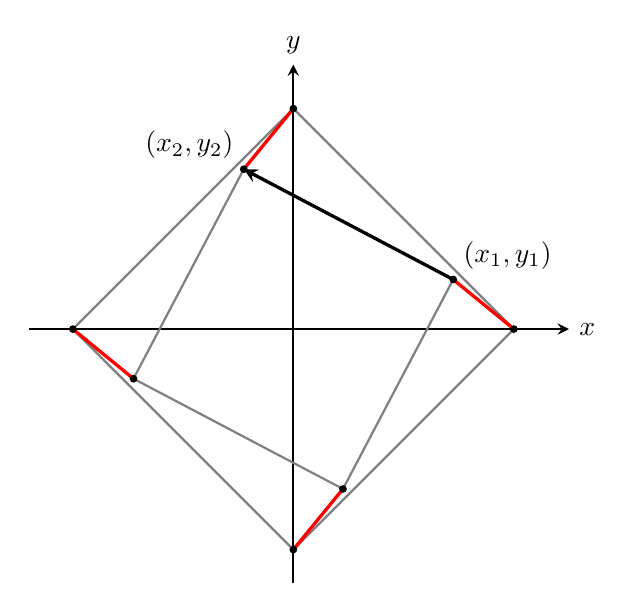
\begin{tikzpicture}[
                          >=stealth,
                          thick,
                          scale=1.4
                      ]

                      % Koordinatenachsen
                      \draw[->] (-2.4,0) -- (2.5,0) node[right] {\(x\)};
                      \draw[->] (0,-2.3) -- (0,2.4) node[above] {\(y\)};

                      % Aeusseres Quadrat
                      \coordinate (A) at (0,2);
                      \coordinate (B) at (2,0);
                      \coordinate (C) at (0,-2);
                      \coordinate (D) at (-2,0);

                      \draw[gray] (A) -- (B) -- (C) -- (D) -- cycle;

                      % Positionen der Hunde nach einer gewissen Zeit
                      \coordinate (H1) at (1.45,0.45);
                      \coordinate (H2) at (-0.45,1.45);
                      \coordinate (H3) at (-1.45,-0.45);
                      \coordinate (H4) at (0.45,-1.45);

                      % Inneres Quadrat
                      \draw[gray] (H1) -- (H2) -- (H3) -- (H4) -- cycle;

                      % Bisherige Bewegungen
                      \draw[red,very thick] (B) -- (H1);
                      \draw[red,very thick] (A) -- (H2);
                      \draw[red,very thick] (D) -- (H3);
                      \draw[red,very thick] (C) -- (H4);

                      % Bewegungsrichtung
                      \draw[->,very thick] (H1) -- (H2) ;

                      % Eckpunkte
                      \foreach \P in {A,B,C,D}
                      \fill (\P) circle (1pt);

                      % Hunde
                      \foreach \P in {H1, H2, H3, H4}
                      \fill (\P) circle (1pt);

                      % Beschriftungen
                      \node[above right] at (H1) {\((x_1,y_1)\)};
                      \node[above left] at (H2) {\((x_2,y_2)\)};

                  \end{tikzpicture}
              \end{center}

              Da die Bahn von Hund Nr.~2 um \(90^\circ\) verdreht ist,
              gilt für dessen Bahn:
              \[
                  \begin{pmatrix}
                      x_2(t) \\y_2(t)
                  \end{pmatrix}
                  =
                  \begin{pmatrix}
                      -y_1(t) \\x_1(t)
                  \end{pmatrix}.
              \]

              Die Geschwindigkeit von Hund Nr.~1 ist gleich dem Vektor
              von Hund Nr.~1 zu Hund Nr.~2, also
              \[
                  \begin{aligned}
                      \frac{\mathrm{d}}{\mathrm{d}t}
                      \begin{pmatrix}x_1\\y_1\end{pmatrix}
                       & =
                      \begin{pmatrix}x_2\\y_2\end{pmatrix}
                      -
                      \begin{pmatrix}x_1\\y_1\end{pmatrix} \\
                       & =
                      \begin{pmatrix}-y_1\\x_1\end{pmatrix}
                      -
                      \begin{pmatrix}x_1\\y_1\end{pmatrix} \\
                       & =
                      \begin{pmatrix}
                          -x_1-y_1 \\
                          x_1-y_1
                      \end{pmatrix}.
                  \end{aligned}
              \]

              \begin{enumerate}
                  \item Lösen Sie das Differentialgleichungssystem
                        zur Anfangsbedingung
                        \[
                            \begin{pmatrix}
                                x_1(0) \\y_1(0)
                            \end{pmatrix}
                            =
                            \begin{pmatrix}1\\0\end{pmatrix}.
                        \]

                  \item Berechnen Sie die Bogenlänge der gesamten Bahn
                        (\(t\to\infty\)).
              \end{enumerate}

        \item \textbf{Windgeschwindigkeitsverlauf.}

              Der Windgeschwindigkeitsverlauf \(\vec{w}(t)\) und damit
              auch die Bahn \(\vec{r}(t)\) eines Luftpartikels werden
              massgeblich durch die Corioliskraft beeinflusst.
              Für die folgenden Berechnungen wird vorausgesetzt,
              dass im betrachteten Gebiet konstanter Druck herrscht
              und die Reibung vernachlässigt werden kann.

              Wir betrachten ein Luftpaket, das sich zum Zeitpunkt
              \(t=0\) an einem Punkt \(P\) der Erdoberfläche befindet
              und dessen Anfangsgeschwindigkeit \(\vec{v}_0\)
              in Richtung Norden zeigt.

              Das Koordinatensystem sei so gewählt, dass der Ursprung
              mit \(P\) übereinstimmt und die horizontale \(u\)-Achse
              nach Osten und die vertikale \(v\)-Achse nach Norden
              ausgerichtet sind.

              \[
                  \vec{w}(t)=
                  \begin{pmatrix}u(t)\\v(t)\end{pmatrix},
                  \qquad
                  \vec{w}(0)=
                  \begin{pmatrix}0\\v_0\end{pmatrix}.
              \]

              Das Gesetz für die Coriolisbeschleunigung für die
              geografische Breite \(\varphi\) lautet
              \[
                  \frac{\mathrm{d}}{\mathrm{d}t}
                  \begin{pmatrix}u(t)\\v(t)\end{pmatrix}
                  =
                  \begin{pmatrix}
                      f\cdot v(t) \\
                      -f\cdot u(t)
                  \end{pmatrix},
              \]
              wobei
              \[
                  f=2\Omega\sin(\varphi),
                  \qquad
                  \Omega=\frac{2\pi}{\SI{86164}{\second}}
              \]
              die Winkelgeschwindigkeit der Erdrotation bezeichnet.

              \begin{enumerate}
                  \item Berechnen Sie die Lösung des
                        Differentialgleichungssystems.
                        Sie können annehmen, dass die geografische
                        Breite \(\varphi\) näherungsweise konstant bleibt.

                  \item Bestimmen Sie eine Gleichung für die Bahn
                        \(\vec{r}(t)\).

                  \item Wir betrachten ein Luftpaket über Winterthur
                        (\(\varphi\approx47^\circ\)) mit der
                        Anfangsgeschwindigkeit
                        \(v_0=\SI{10}{\meter\per\second}\).

                        Wie lange dauert es, bis das Luftpaket gemäss
                        obigem Modell wieder über Winterthur ist?

                        Welche Strecke hat es in dieser Zeit zurückgelegt?
              \end{enumerate}
    \end{enumerate}

\end{ueb}

\clearpage
\textbf{Lösungen}

\begin{enumerate}
    \item Die entsprechende Matrix
          \[
              A=\begin{pmatrix}
                  4  & 1 \\
                  -4 & 0
              \end{pmatrix}
          \]
          hat nur einen Eigenwert \(\lambda=2\) und einen
          eindimensionalen Eigenraum mit dem Eigenvektor
          \[
              \vec{v}=\begin{pmatrix}1\\-2\end{pmatrix}.
          \]

          Die allgemeine Lösung lautet
          \[
              \vec{x}(t)=e^{2t}
              \left(
              c_1\begin{pmatrix}1\\-2\end{pmatrix}
              +c_2\begin{pmatrix}t\\-2t+1\end{pmatrix}
              \right).
          \]

          Mit den Anfangsbedingungen erhält man:
          \[
              \boxed{
                  x_1(t)=2e^{2t}+5te^{2t},
                  \qquad
                  x_2(t)=e^{2t}-10te^{2t}
              }
          \]

    \item \textbf{Hunde}

          Die Matrix
          \[
              A=\begin{pmatrix}
                  -1 & -1 \\
                  1  & -1
              \end{pmatrix}
          \]
          hat die Eigenwerte
          \[
              \lambda_1=-1+i,\qquad
              \lambda_2=-1-i
          \]
          mit den zugehörigen Eigenvektoren
          \[
              \vec{v}_1=\begin{pmatrix}1\\-i\end{pmatrix},
              \qquad
              \vec{v}_2=\begin{pmatrix}1\\i\end{pmatrix}.
          \]

          Aus der komplexen Lösung kann die reelle Lösung
          \[
              \begin{pmatrix}x_1(t)\\y_1(t)\end{pmatrix}
              =
              e^{-t}\left[
                  c_1
                  \begin{pmatrix}\cos t\\\sin t\end{pmatrix}
                  +
                  c_2
                  \begin{pmatrix}\sin t\\-\cos t\end{pmatrix}
                  \right]
          \]
          ermittelt werden.

          Mit den Anfangsbedingungen findet man:
          \[
              \boxed{
                  \begin{pmatrix}x_1(t)\\y_1(t)\end{pmatrix}
                  =
                  e^{-t}
                  \begin{pmatrix}\cos t\\\sin t\end{pmatrix}
              }
          \]

          Die Bahn ist eine sogenannte \emph{logarithmische Spirale}.
          Sie windet sich unendlich oft um den Ursprung des
          Koordinatensystems.

          Ihre Gesamtlänge ist aber endlich:
          \[
              \begin{aligned}
                  l
                   & =\int_0^\infty
                  \sqrt{\dot{x}_1(t)^2+\dot{y}_1(t)^2}\,\mathrm{d}t \\
                   & =\int_0^\infty \sqrt{2}\,e^{-t}\,\mathrm{d}t   \\
                   & =\boxed{\sqrt{2}}.
              \end{aligned}
          \]

    \item \textbf{Wind}

          Die Matrix
          \[
              A=\begin{pmatrix}
                  0  & f \\
                  -f & 0
              \end{pmatrix}
          \]
          hat die Eigenwerte
          \[
              \lambda_{1,2}=\pm fi
          \]
          mit den zugehörigen Eigenvektoren
          \[
              \vec{v}_{1,2}=
              \begin{pmatrix}1\\\pm i\end{pmatrix}.
          \]

          Die allgemeine reelle Lösung lautet
          \[
              \vec{w}(t)
              =
              c_1\begin{pmatrix}
                  \cos(ft) \\-\sin(ft)
              \end{pmatrix}
              +
              c_2\begin{pmatrix}
                  \sin(ft) \\\cos(ft)
              \end{pmatrix}.
          \]

          Mit den Anfangsbedingungen folgt:
          \[
              \boxed{
                  \vec{w}(t)=v_0
                  \begin{pmatrix}
                      \sin(ft) \\
                      \cos(ft)
                  \end{pmatrix}
              }
          \]

          Durch Integrieren und Berücksichtigung von
          \(\vec{r}(0)=\vec{0}\) erhält man:
          \[
              \begin{aligned}
                  \vec{r}(t)
                   & =\frac{v_0}{f}
                  \begin{pmatrix}
                      1-\cos(ft) \\
                      \sin(ft)
                  \end{pmatrix} \\[2mm]
                   & =
                  \begin{pmatrix}
                      \frac{v_0}{f} \\0
                  \end{pmatrix}
                  +
                  \frac{v_0}{f}
                  \begin{pmatrix}
                      -\cos(ft) \\
                      \sin(ft)
                  \end{pmatrix}.
              \end{aligned}
          \]

          Die Bahn beschreibt einen Kreis mit Radius
          \(
          \boxed{R=\frac{v_0}{f}}.
          \)
          \begin{center}
              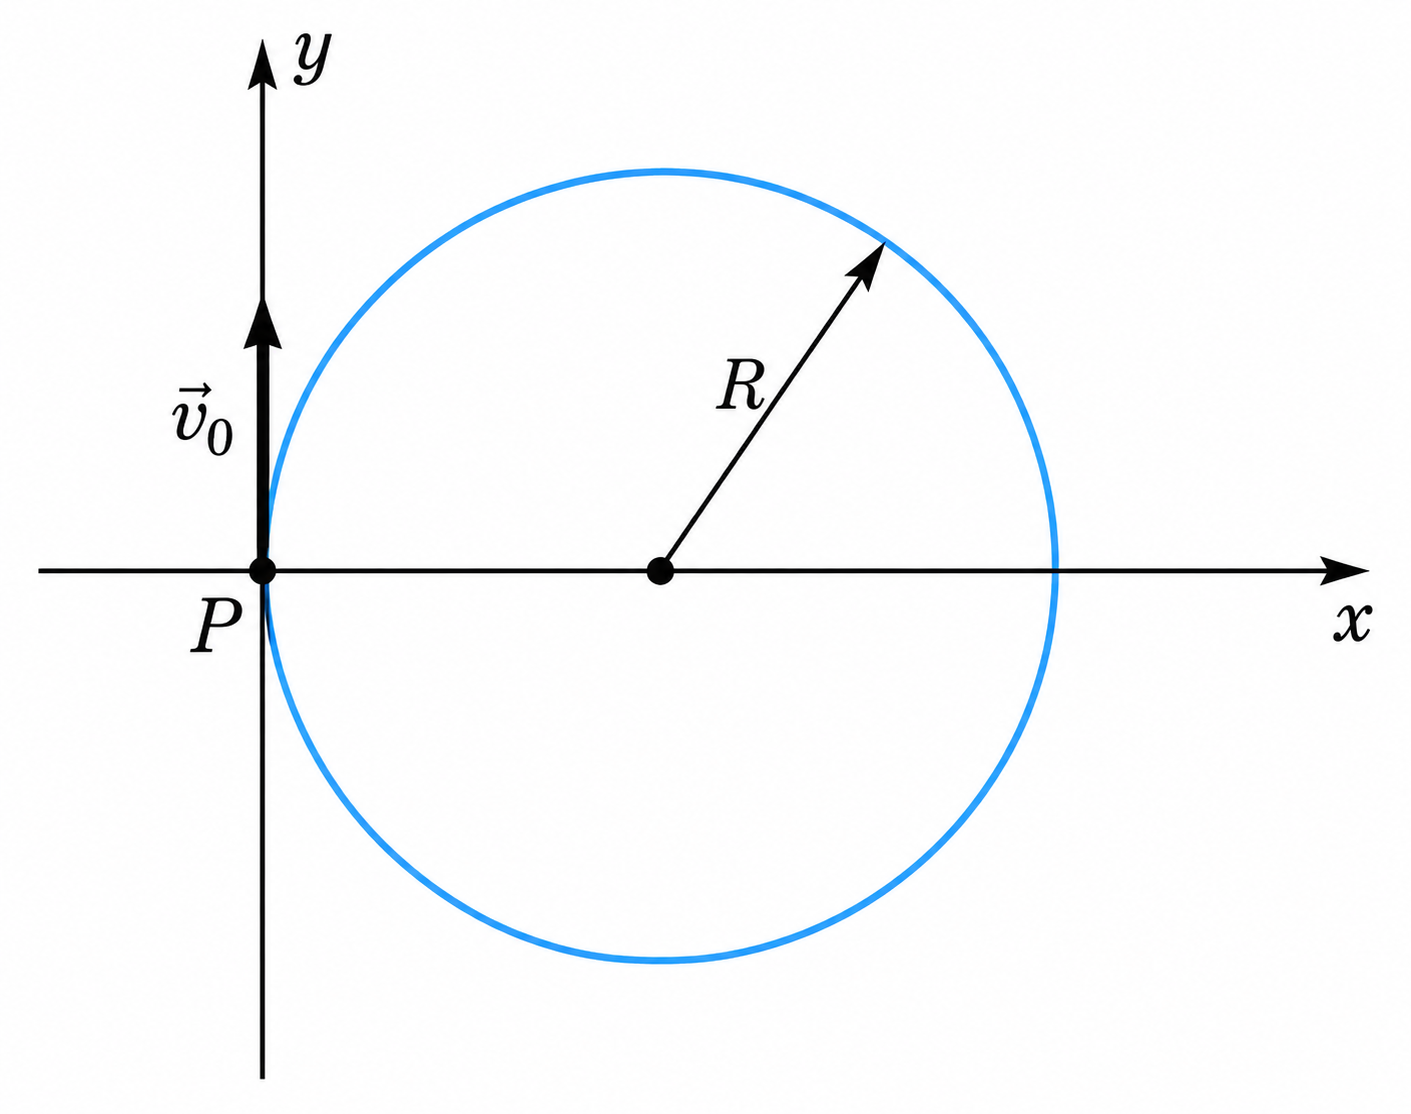
\includegraphics[width = 0.25\textwidth]{media/WindBahn.png}
          \end{center}

          Die Umlaufzeit beträgt
          \(
          T=\frac{2\pi}{f}.
          \)

          Für das Luftpaket über Winterthur gilt
          \[
              f=2\Omega\sin(\varphi)
              \approx \SI{1.064e-4}{\per\second}.
          \]

          Damit erhält man
          \[
              R=\frac{10}{f}\approx\SI{94.0}{\kilo\meter}.
          \]

          Die gesamte zurückgelegte Strecke beträgt
          \[
              \boxed{
                  L=2\pi R\approx\SI{590.7}{\kilo\meter}
              }.
          \]

          Die Umlaufzeit beträgt
          \[
              \boxed{
                  T=\frac{2\pi}{f}\approx\SI{16.4}{\hour}
              }.
          \]
\end{enumerate}


























\clearpage
\subsection{Differentialgleichungen 2. Ordnung als Systeme 1. Ordnung}

Wie Ihnen möglicherweise bereits aufgefallen ist, gibt es gewisse Parallelen zwischen homogenen Differentialgleichungen 2. Ordnung, deren Lösungen wir mithilfe einer charakteristischen Gleichung bestimmt haben, und homogenen Differentialgleichungssystemen.

Tatsächlich lassen sich Differentialgleichungen zweiter oder höherer Ordnung durch Differentialgleichungssysteme 1. Ordnung ausdrücken und lösen.

Sei zum Beispiel die Differentialgleichung
\[
    \ddot{x}+5\dot{x}+6x=0
\]
gegeben. Wie wir bereits wissen, lautet die allgemeine Lösung
\[
    x(t)=c_1e^{-2t}+c_2e^{-3t},
\]
da die charakteristische Gleichung
\[
    \lambda^2+5\lambda+6=0
\]
die Lösungen \(\lambda_1=-2\) und \(\lambda_2=-3\) hat.

Wie könnte man nun die Differentialgleichung
\[
    \ddot{x}+5\dot{x}+6x=0
\]
durch ein Differentialgleichungssystem 1. Ordnung ausdrücken?

Folgender Trick ermöglicht genau dies:
Wir definieren
\[
    x_1=x
    \qquad\text{und}\qquad
    x_2=\dot{x}.
\]

\karofeld{5}
% Damit folgt:
% \[
%     \begin{aligned}
%         \dot{x}_1 & = x_2,     \\
%         \dot{x}_2 & = \ddot{x}
%         = -6x-5\dot{x}
%         = -6x_1-5x_2.
%     \end{aligned}
% \]

% Wir erhalten somit das Differentialgleichungssystem
% \[
%     \boxed{
%         \frac{d}{dt}
%         \begin{pmatrix}
%             x_1 \\
%             x_2
%         \end{pmatrix}
%         =
%         \begin{pmatrix}
%             0  & 1  \\
%             -6 & -5
%         \end{pmatrix}
%         \begin{pmatrix}
%             x_1 \\
%             x_2
%         \end{pmatrix}
%     }
% \]
\clearpage
\begin{ueb}{Differentialgleichungen 2. Ordnung als Systeme 1. Ordnung}{}
    \begin{enumerate}
        \item Lösen Sie das obige Differentialgleichungssystem und
              vergleichen Sie die Lösung mit der bereits bekannten
              Lösung der Differentialgleichung 2. Ordnung.

        \item Lösen Sie die folgenden Differentialgleichungen,
              indem Sie diese zunächst durch ein
              Differentialgleichungssystem 1. Ordnung ausdrücken.

              \begin{enumerate}
                  \item \(\ddot{x}-5\dot{x}+4x=0\)
                  \item \(\ddot{x}+x=0\)
                  \item \(\dddot{x}-3\ddot{x}-4\dot{x}=0\)
              \end{enumerate}
    \end{enumerate}
\end{ueb}

\clearpage
\textbf{Lösungen:}

\begin{enumerate}
    \item
          \[
              x(t)=c_1e^{-2t}+c_2e^{-3t}
          \]

    \item
          \begin{enumerate}
              \item
                    \[
                        x(t)=c_1e^t+c_2e^{4t}
                    \]

              \item
                    Die Eigenwerte der Matrix sind \(\lambda_{1,2}=\pm i\)
                    mit den zugehörigen Eigenvektoren
                    \[
                        \vec{v}_1=\begin{pmatrix}1\\i\end{pmatrix},
                        \qquad
                        \vec{v}_2=\begin{pmatrix}1\\-i\end{pmatrix}.
                    \]
                    Die allgemeine reelle Lösung lautet:
                    \[
                        x(t)=c_1\cos(t)+c_2\sin(t)
                    \]

              \item
                    Setzen wir \(y=\dot{x}\), so erhalten wir eine
                    Differentialgleichung 2. Ordnung:
                    \[
                        \ddot{y}-3\dot{y}-4y=0.
                    \]
                    Ihre allgemeine Lösung lautet
                    \[
                        y(t)=c_1e^{-t}+c_2e^{4t}.
                    \]
                    Durch Integration folgt:
                    \[
                        \begin{aligned}
                            x(t)
                             & = -c_1e^{-t}+\frac{c_2}{4}e^{4t}+c_3 \\
                             & = c_1^*e^{-t}+c_2^*e^{4t}+c_3.
                        \end{aligned}
                    \]
          \end{enumerate}
\end{enumerate}


























\clearpage
\subsection{Inhomogene lineare Differentialgleichungssysteme erster Ordnung}

Betrachten wir nun lineare Differentialgleichungssysteme erster Ordnung mit Inhomogenitäten:

\[
    \frac{d}{dt}\vec{x}=A\vec{x}+\vec{b}
\]

\begin{satz}{Allgemeine Lösung eines inhomogenen Differentialgleichungssystems}{}
    Die allgemeine Lösung des inhomogenen Differentialgleichungssystems
    \[
        \frac{d}{dt}\vec{x}=A\vec{x}+\vec{b}
    \]
    erhält man, indem man eine sogenannte \textbf{partikuläre Lösung}
    \(\vec{x}_p\) bestimmt und zu ihr die allgemeine Lösung
    \(\vec{x}_h\) des zugehörigen homogenen Differentialgleichungssystems
    addiert:

    \[
        \vec{x}(t)=\vec{x}_p(t)+\vec{x}_h(t)
    \]
\end{satz}

\begin{bsp}{Variation der Konstanten bei DGL-Systemen}{}

    Wir betrachten das inhomogene Differentialgleichungssystem
    \[
        \begin{pmatrix}
            \dot{x}_1 \\
            \dot{x}_2
        \end{pmatrix}
        =
        \begin{pmatrix}
            1 & 1 \\
            4 & 1
        \end{pmatrix}
        \begin{pmatrix}
            x_1 \\
            x_2
        \end{pmatrix}
        +
        \begin{pmatrix}
            2 \\
            -1
        \end{pmatrix}e^t.
    \]

    Die zugehörige homogene Gleichung lautet
    \[
        \begin{pmatrix}
            \dot{x}_1 \\
            \dot{x}_2
        \end{pmatrix}
        =
        \begin{pmatrix}
            1 & 1 \\
            4 & 1
        \end{pmatrix}
        \begin{pmatrix}
            x_1 \\
            x_2
        \end{pmatrix}.
    \]

    Die Matrix
    \[
        A=\begin{pmatrix}
            1 & 1 \\
            4 & 1
        \end{pmatrix}
    \]
    besitzt die Eigenwerte \(\lambda_1=3\) und \(\lambda_2=-1\)
    mit den zugehörigen Eigenvektoren
    \[
        \vec{v}_1=\begin{pmatrix}1\\2\end{pmatrix},
        \qquad
        \vec{v}_2=\begin{pmatrix}1\\-2\end{pmatrix}.
    \]

    Die allgemeine Lösung des homogenen Systems lautet somit
    \[
        \vec{x}_h(t)
        =
        c_1\begin{pmatrix}1\\2\end{pmatrix}e^{3t}
        +
        c_2\begin{pmatrix}1\\-2\end{pmatrix}e^{-t}.
    \]

    Die partikuläre Lösung kann wie bei gewöhnlichen
    Differentialgleichungen mithilfe der
    \textbf{Variation der Konstanten} bestimmt werden.

    Dazu schreiben wir die homogene Lösung zunächst in Matrixform:
    \[
        \begin{aligned}
            \vec{x}_h(t)
             & =
            c_1\begin{pmatrix}1\\2\end{pmatrix}e^{3t}
            +
            c_2\begin{pmatrix}1\\-2\end{pmatrix}e^{-t} \\[2mm]
             & =
            \underbrace{
                \begin{pmatrix}
                    e^{3t}  & e^{-t}   \\
                    2e^{3t} & -2e^{-t}
                \end{pmatrix}
            }_{X(t)}
            \underbrace{
                \begin{pmatrix}
                    c_1 \\c_2
                \end{pmatrix}
            }_{\vec{c}}.
        \end{aligned}
    \]

    Dabei nennt man \(X(t)\) eine Fundamentalmatrix des homogenen Systems.

    Nun beginnt die Variation der Konstanten.
    Wir ersetzen die Konstanten \(c_1,c_2\) durch Funktionen
    \(c_1(t),c_2(t)\) und verwenden den Ansatz
    \[
        \vec{x}(t)
        =
        \begin{pmatrix}
            e^{3t}  & e^{-t}   \\
            2e^{3t} & -2e^{-t}
        \end{pmatrix}
        \begin{pmatrix}
            c_1(t) \\c_2(t)
        \end{pmatrix}
        =
        X(t)\vec{c}(t).
    \]

    Diesen Ansatz setzen wir in die Differentialgleichung ein:
    \[
        \frac{d}{dt}\bigl(X(t)\vec{c}(t)\bigr)
        =
        AX(t)\vec{c}(t)
        +
        \begin{pmatrix}2\\-1\end{pmatrix}e^t.
    \]

    Die Ableitung von \(X(t)\vec{c}(t)\) kann mithilfe
    der Produktregel ermittelt werden:
    \[
        \underbrace{\dot{X}(t)}_{AX(t)}\vec{c}(t)
        +
        X(t)\dot{\vec{c}}(t)
        =
        AX(t)\vec{c}(t)
        +
        \begin{pmatrix}2\\-1\end{pmatrix}e^t.
    \]

    Analog zur Variation der Konstanten im eindimensionalen Fall
    heben sich zwei Terme auf. Durch Multiplikation von links
    mit \(X(t)^{-1}\) erhalten wir:
    \[
        \begin{aligned}
            \dot{\vec{c}}(t)
             & =
            X(t)^{-1}
            \begin{pmatrix}2\\-1\end{pmatrix}e^t \\[2mm]
             & =
            \begin{pmatrix}
                e^{3t}  & e^{-t}   \\
                2e^{3t} & -2e^{-t}
            \end{pmatrix}^{-1}
            \begin{pmatrix}
                2e^t \\-e^t
            \end{pmatrix}                   \\[2mm]
             & =
            \frac{1}{-4e^{2t}}
            \begin{pmatrix}
                -2e^{-t} & -e^{-t} \\
                -2e^{3t} & e^{3t}
            \end{pmatrix}
            \begin{pmatrix}
                2e^t \\-e^t
            \end{pmatrix}                   \\[2mm]
             & =
            \frac{1}{-4e^{2t}}
            \begin{pmatrix}
                -4+1 \\
                -4e^{4t}-e^{4t}
            \end{pmatrix}                   \\[2mm]
             & =
            \begin{pmatrix}
                \frac34 e^{-2t} \\[1mm]
                \frac54 e^{2t}
            \end{pmatrix}.
        \end{aligned}
    \]

    Durch Integration können wir nun \(\vec{c}(t)\) bestimmen:
    \[
        \vec{c}(t)
        =
        \begin{pmatrix}
            -\frac38 e^{-2t}+c_1 \\[2mm]
            \frac58 e^{2t}+c_2
        \end{pmatrix}.
    \]

    Damit lautet die allgemeine Lösung:
    \[
        \begin{aligned}
            \begin{pmatrix}x_1\\x_2\end{pmatrix}
             & =
            \begin{pmatrix}
                e^{3t}  & e^{-t}   \\
                2e^{3t} & -2e^{-t}
            \end{pmatrix}
            \begin{pmatrix}
                -\frac38 e^{-2t}+c_1 \\[1mm]
                \frac58 e^{2t}+c_2
            \end{pmatrix}            \\[3mm]
             & =
            \begin{pmatrix}
                e^{3t}  & e^{-t}   \\
                2e^{3t} & -2e^{-t}
            \end{pmatrix}
            \begin{pmatrix}
                -\frac38 e^{-2t} \\[1mm]
                \frac58 e^{2t}
            \end{pmatrix}
            +
            \underbrace{
                \begin{pmatrix}
                    e^{3t}  & e^{-t}   \\
                    2e^{3t} & -2e^{-t}
                \end{pmatrix}
                \begin{pmatrix}c_1\\c_2\end{pmatrix}
            }_{\vec{x}_h(t)}    \\[3mm]
             & =
            \begin{pmatrix}
                -\frac38 e^t+\frac58 e^t \\[1mm]
                -\frac34 e^t-\frac54 e^t
            \end{pmatrix}
            +
            c_1\begin{pmatrix}1\\2\end{pmatrix}e^{3t}
            +
            c_2\begin{pmatrix}1\\-2\end{pmatrix}e^{-t} \\[3mm]
             & =
            \boxed{
                \begin{pmatrix}
                    \frac14 \\-2
                \end{pmatrix}e^t
                +
                c_1\begin{pmatrix}1\\2\end{pmatrix}e^{3t}
                +
                c_2\begin{pmatrix}1\\-2\end{pmatrix}e^{-t}
            }.
        \end{aligned}
    \]

\end{bsp}

Wie Sie sehen, ist die Variation der Konstanten für
Differentialgleichungssysteme recht aufwendig. Häufig wird deshalb
eine andere Methode verwendet, bei der man versucht, die Form
einer partikulären Lösung zu erraten.

In unserem Beispiel bietet sich aufgrund der Inhomogenität
\[
    \vec b(t)=
    \begin{pmatrix}
        2e^t \\
        -e^t
    \end{pmatrix}
\]
der Ansatz
\[
    \vec x_p(t)=
    \begin{pmatrix}
        ae^t \\
        be^t
    \end{pmatrix}
\]
an.

Durch Einsetzen in das Differentialgleichungssystem erhält man
\[
    \begin{pmatrix}
        ae^t \\
        be^t
    \end{pmatrix}
    =
    \begin{pmatrix}
        1 & 1 \\
        4 & 1
    \end{pmatrix}
    \begin{pmatrix}
        ae^t \\
        be^t
    \end{pmatrix}
    +
    \begin{pmatrix}
        2e^t \\
        -e^t
    \end{pmatrix}.
\]

Nach Division durch \(e^t\) ergibt sich das lineare Gleichungssystem
\[
    \begin{aligned}
        a & = a+b+2,  \\
        b & = 4a+b-1.
    \end{aligned}
\]

Daraus folgen die Koeffizienten
\[
    \boxed{a=\frac14,\qquad b=-2.}
\]

Somit lautet eine partikuläre Lösung
\[
    \boxed{
        \vec x_p(t)=
        \begin{pmatrix}
            \frac14 \\
            -2
        \end{pmatrix}e^t.
    }
\]
\clearpage
\begin{ueb}{Zwei verbundene Behälter}{}

    Als Einführung in dieses Kapitel haben wir zwei verbundene
    Behälter betrachtet, die beide ein Gemisch aus Farbstoff und
    Wasser enthielten. Dies führte auf das Differentialgleichungssystem
    \[
        \begin{pmatrix}
            \dot{x}_1 \\
            \dot{x}_2
        \end{pmatrix}
        =
        \begin{pmatrix}
            -\frac{1}{25} & \frac{3}{100} \\
            \frac{1}{25}  & -\frac{1}{20}
        \end{pmatrix}
        \begin{pmatrix}
            x_1 \\
            x_2
        \end{pmatrix}
        +
        \begin{pmatrix}
            1 \\
            0
        \end{pmatrix}
    \]
    mit den Anfangsbedingungen \(x_1(0)=x_2(0)=0\).

    \begin{enumerate}
        \item Lösen Sie das zugehörige homogene
              Differentialgleichungssystem.

        \item Wegen der negativen Eigenwerte können wir davon
              ausgehen, dass sich die Farbstoffkonzentrationen
              einem stabilen Endzustand nähern. Damit ist der
              Ansatz
              \[
                  \vec{x}_p=
                  \begin{pmatrix}
                      a \\
                      b
                  \end{pmatrix}
              \]
              für eine partikuläre Lösung plausibel.

              Setzen Sie \(\vec{x}_p\) in das
              Differentialgleichungssystem ein und bestimmen Sie
              die beiden Zahlen \(a\) und \(b\).

              Wie lautet die Lösung des Differentialgleichungssystems
              unter Berücksichtigung der Anfangsbedingungen?

        \item Bestimmen Sie die allgemeine Lösung des inhomogenen
              Differentialgleichungssystems mithilfe der
              Variation der Konstanten.
    \end{enumerate}

\end{ueb}
\clearpage
\textbf{Lösungen}
\begin{enumerate}
    \item Die Eigenwerte und zugehörigen Eigenvektoren sind
          \[
              \lambda_1=-\frac{1}{100},
              \qquad
              \vec v_1=\begin{pmatrix}1\\1\end{pmatrix},
              \qquad
              \lambda_2=-\frac{8}{100},
              \qquad
              \vec v_2=\begin{pmatrix}-3\\4\end{pmatrix}.
          \]
          Damit lautet die allgemeine Lösung des homogenen Systems
          \[
              \boxed{
                  \vec x_h(t)
                  =c_1\begin{pmatrix}1\\1\end{pmatrix}e^{-t/100}
                  +c_2\begin{pmatrix}-3\\4\end{pmatrix}e^{-8t/100}.
              }
          \]

    \item Einsetzen des konstanten Ansatzes
          \[
              \vec x_p=\begin{pmatrix}a\\b\end{pmatrix}
          \]
          in das Differentialgleichungssystem liefert
          \[
              \begin{cases}
                  -\dfrac{1}{25}a+\dfrac{3}{100}b+1=0, \\[2mm]
                  \dfrac{1}{25}a-\dfrac{1}{20}b=0.
              \end{cases}
          \]
          Daraus folgt
          \[
              a=\frac{125}{2},
              \qquad b=50.
          \]
          Eine partikuläre Lösung ist somit
          \[
              \vec x_p=\frac12\begin{pmatrix}125\\100\end{pmatrix}.
          \]

          Die allgemeine Lösung des inhomogenen Systems lautet
          \[
              \vec x(t)
              =c_1\begin{pmatrix}1\\1\end{pmatrix}e^{-t/100}
              +c_2\begin{pmatrix}-3\\4\end{pmatrix}e^{-8t/100}
              +\frac12\begin{pmatrix}125\\100\end{pmatrix}.
          \]

          Mit den Anfangsbedingungen \(x_1(0)=x_2(0)=0\)
          erhalten wir
          \[
              \begin{cases}
                  c_1-3c_2+\dfrac{125}{2}=0, \\[2mm]
                  c_1+4c_2+50=0.
              \end{cases}
          \]
          Daraus ergeben sich
          \[
              c_1=-\frac{400}{7},
              \qquad
              c_2=\frac{25}{14}.
          \]

          Die gesuchte Lösung ist also
          \[
              \boxed{
                  \vec x(t)
                  =-\frac{400}{7}
                  \begin{pmatrix}1\\1\end{pmatrix}e^{-t/100}
                  +\frac{25}{14}
                  \begin{pmatrix}-3\\4\end{pmatrix}e^{-8t/100}
                  +\frac12\begin{pmatrix}125\\100\end{pmatrix}.
              }
          \]

    \item Die Fundamentalmatrix des homogenen Systems lautet
          \[
              X(t)=
              \begin{pmatrix}
                  e^{-t/100} & -3e^{-8t/100} \\
                  e^{-t/100} & 4e^{-8t/100}
              \end{pmatrix}.
          \]
          Mit dem Ansatz
          \[
              \vec x(t)=X(t)\vec c(t)
          \]
          ergibt die Variation der Konstanten
          \[
              \vec c'(t)
              =X(t)^{-1}\begin{pmatrix}1\\0\end{pmatrix}.
          \]

          Wegen
          \[
              X(t)^{-1}
              =\frac17
              \begin{pmatrix}
                  4e^{t/100}  & 3e^{t/100} \\
                  -e^{8t/100} & e^{8t/100}
              \end{pmatrix}
          \]
          folgt
          \[
              \vec c'(t)
              =\begin{pmatrix}
                  \frac47 e^{t/100} \\[1mm]
                  -\frac17 e^{8t/100}
              \end{pmatrix}.
          \]

          Durch Integration erhalten wir
          \[
              \vec c(t)=
              \begin{pmatrix}
                  \frac{400}{7}e^{t/100}+c_1 \\[1mm]
                  -\frac{25}{14}e^{8t/100}+c_2
              \end{pmatrix}.
          \]

          Einsetzen in \(\vec x(t)=X(t)\vec c(t)\) liefert
          schliesslich
          \[
              \boxed{
                  \vec x(t)
                  =c_1\begin{pmatrix}1\\1\end{pmatrix}e^{-t/100}
                  +c_2\begin{pmatrix}-3\\4\end{pmatrix}e^{-8t/100}
                  +\frac12\begin{pmatrix}125\\100\end{pmatrix}.
              }
          \]
\end{enumerate}
